\documentclass[12pt]{article}
\usepackage[total={170mm,230mm}]{geometry}

\usepackage{cmap}
\usepackage{hyperref}
\usepackage[utf8]{inputenc}
\usepackage[T2A]{fontenc}
\usepackage[russian]{babel}

\usepackage{graphicx}
\usepackage{listings}
\usepackage{xcolor}
\usepackage{color}
\usepackage{amssymb}
\usepackage{amsfonts}
\usepackage{amsmath}
\usepackage{amsthm}
\usepackage{physics}
\usepackage{wrapfig}
\usepackage{cancel}
\usepackage{pdfpages}
\usepackage{hyperref}
\usepackage{multirow}
\usepackage{adjustbox}

\lstset{%
  frame=tlrb,%      the frame is open on the right side
  resetmargins=false,%
  rulesepcolor=\color{black},%
  numbers=left,%                % left
  numberstyle=\tiny,%
  numbersep=5pt,%
  firstnumber=1,%
  stepnumber=5,%
  columns=fixed,%               % to prevent inserting spaces
  fontadjust=true,%
  keepspaces=true,%
  basewidth=0.5em,%
  captionpos=t,%
  abovecaptionskip=\smallskipamount,% same amount as defaul_t
  belowcaptionskip=\smallskipamount,% in caption package
}
\lstdefinestyle{fortran}{%
  backgroundcolor=\color{yellow!10},%
  basicstyle=\small\ttfamily,%
  identifierstyle=\color{black},%
  keywordstyle=\color{blue},%
  keywordstyle={[2]\color{cyan}},%
  keywordstyle={[3]\color{olive}},%
  stringstyle=\color{teal},%
  commentstyle=\itshape\color{orange},%
}%

% \numberwithin{equation}{section}

\newtheorem{definition}{Опредление}[section]
\newtheorem{theorem}{Теорема}[section]
\newtheorem{axiom}{Аксиома}[section]

\usepackage{pgfplots}
\pgfplotsset{width=7cm,compat=newest}

\usepackage{amsmath}
\DeclareMathOperator\arctanh{arctanh}

\usepackage{amsmath}
\DeclareMathOperator\arccosh{arccosh}

\usepackage{amsmath}
\DeclareMathOperator\const{const}

\begin{document}

%!TEX
\begin{titlepage}
	\begin{center}
	% \vspace{-3em}
	{\textsc{Санкт-Петербургский государственный университет}}
	\vskip 2pt \hrule \vskip 3pt
	{\textsc{Физический факультет}}

	\vfill


	{\Large \bfseries ЗАДАНИЕ В}

		
	\vspace{2cm}
	{\large Работу выполнил студент \\[0.5em]{\Large \bfseries Козлов Александр}}

	\end{center}

	\vfill

	\begin{center}
	{Санкт-Петербург, \today}
	\end{center}
\end{titlepage}
\setcounter{page}{2}

\tableofcontents
\newpage

\section*{Формулировка задания}

СЛАУ:
\begin{equation}
    \label{eq:1}
    \vb{A} \vb{x} = \vb{b}^{(i)},\; i=1,2,\ldots,10.
\end{equation}
Матрица $\vb{A}$ симметричная и положительно определенная. Оптимизировать программную реализацию решателя этой системы, основанного на разложении Холецкого, используя OpenMP. Исследовать зависимость масштабируемости параллельной версии программы от ее вычислительной трудоемкости.

Проверка закона Амдала. Построить зависимость ускорение: число потоков для заданного примера.

\section{Описание программно-аппаратной конфигурации тестового стенда}

В качестве тестового стенда выступала вычислительная машина, доступ к которому был предоставлен преподавателем. Краткое описание программно-аппаратной конфигурации тестового стенда приведено в Таблице \ref{tab:1}.
\begin{table}[!ht]
    \centering
    \begin{tabular}{|l|l|}
    \hline
        ОС & Ubuntu 20.04.4 LTS \\ \hline
        Число ядер & 6 \\ \hline
        Число потоков & 12 \\ \hline
        Модель процессора & Intel(R) Xeon(R) E-2136 CPU @ 3.30GHz \\ \hline
        ОЗУ & 62GB \\ \hline
        Компилятор & gfortran \\ \hline
    \end{tabular}
    \caption{Программно-аппаратная конфигурация тестового стенда.}
    \label{tab:1}
\end{table}

\section{Описание метода решения задачи}

\subsection{Описание последовательного алгоритма решения задачи}

Первым этапом решения задачи является применение разложения Холецкого к симметричной и положительно определенной матрице $\vb{A}$, то есть ее представление в виде $\vb{A}=\vb{L}\vb{L}^T$, где матрица $\vb{L}$ --- нижняя треугольная матрица со строго положительными элементами на диагонали. Реализация последовательного алгоритма разложения Холецкого на Фортране в простейшем (без перестановок суммирования) варианте была взята с \href{https://algowiki-project.org/en/Cholesky_decomposition}{сайта проекта AlgoWiki}. Данная реализация представлена в Листинге \ref{listing:1}. Переменная $s$ имеет двойную точность, в то время как остальные --- одинарную.
\begin{lstlisting}[language=fortran, style=fortran, label={listing:1}, caption=Реализация последовательного алгоритма разложения Холецкого на Фортране в простейшем (без перестановок суммирования) варианте.]
do  i = 1, n
   s = l(i,i)
   do  ip = 1, i - 1
      s = s - dprod(l(i,ip), l(i,ip))
   end do
   l(i,i) = sqrt(s)
   do  j = i + 1, n
      s = l(j,i)
      do  ip = 1, i-1
         s = s - dprod(l(i,ip), l(j,ip))
      end do
      l(j,i) = s / l(i,i)
   end do
end do
\end{lstlisting}

Вторым этапом решения задачи является обратная подстановка. То есть последовательно решаются 2 СЛАУ с треугольными матрицами
$$
\begin{cases}
    \vb{L}\vb{y} = \vb{b}^{(i)},\\
    \vb{L}^T\vb{x} = \vb{y}
\end{cases}
$$
для $i=1,2,\ldots,10$. Вектор $\vb{y}$ находится по формулам
$$
y_1 = \dfrac{b^{(i)}_1}{l_{11}};\; y_{j} = \dfrac{b_j^{(i)} - \sum_{p=1}^{j-1} l_{jp} y_p}{l_{jj}},\; j=2,3,\ldots,n,
$$
где $n$ --- число столбцов матрицы $\vb{A}$. Вектор $\vb{x}$ находится аналогично
$$
x_n = \dfrac{y_n}{{l^T}_{nn}};\; x_{j} = \dfrac{y_j - \sum_{p=j+1}^{n} {l^T}_{jp} x_p}{{l^T}_{jj}},\; j=n-1,n-2,\ldots,1.
$$
Последовательный вариант реализации второго этапа решения задачи представлен в Листинге \ref{listing:2}.
\begin{lstlisting}[language=fortran, style=fortran, label={listing:2}, caption=Последовательная реализация обратной подстановки на Фортране.]
do i = 1, m
    y(1) = b(1,i) / l(1,1)
    do j = 2, n
        s = b(j,i)
        do ip = 1, j - 1
            s = s - dprod(l(j,ip), y(ip))
        end do
        y(j) = s / l(j,j)
    end do
    x(n,i) = y(n) / l_t(n,n)
    do j = n - 1, 1, -1
    s = y(j)
        do ip = j + 1, n
            s = s - dprod(l_t(j,ip), x(ip,i)) 
        end do
        x(j,i) = s / l_t(j,j)
    end do
end do
\end{lstlisting}

\subsection{Описание оптимизации с использованием OpenMP}

Исходный код, оптимизированного с помощью OpenMP решателя системы \eqref{eq:1}, основанного на разложении Холецкого, на Фортране приведен в Листинге \ref{listing:3}. Сперва был распараллелен код, отвечающий за декомпозицию Холецкого. Из Листинга \ref{listing:1} видно, что цикл по $j$ не содержит цикловых зависимостей, поэтому он был распараллелен с помощью директивы следующей директивы OpenMP:
\begin{lstlisting}[language=fortran, style=fortran, caption={Директива OpenMP, которая была использована для распараллеливания цикла \texttt{do} при реализации разложения Холецкого}.]
!$omp parallel do private(j,ip,s) shared(l,i) schedule(static)
\end{lstlisting}
Директива \texttt{!\$omp parallel do} помечает цикл \texttt{do}, следующий сразу после данной директивы, чтобы сделать его распараллеливаемым. Число итераций цикла зависит от $j$ и составляет $n-(j+1)$, что означает, что данный цикл может одновременно выполняться не более чем $n-(j+1)$ потоками. Оператор \texttt{private(j,ip,s)} объявляет переменные $j$, $ip$ и $s$ локальными, то есть на каждом потоке создается локальная копия данных переменных. Оператор \texttt{shared(l,i)} объявляет переменные $l$ и $i$ общими для потоков. Оператор \texttt{schedule(static)} задает такой способ распределения итераций цикла между потоками, что количество итераций цикла, передаваемых для выполнения каждому потоку, фиксировано (в данном случае равно 1) и распределяется между нитями по принципу кругового планирования.

Далее была распараллелена часть решателя, отвечающая обратной подстановке. Цикл \texttt{do} по $i$, как можно заметить из Листинга \ref{listing:2}, не содержит цикловых зависимостей, поэтому он и был выбран для распаралелливания. Для этого перед началом данного цикла была помещена директива: 
\begin{lstlisting}[language=fortran, style=fortran, caption={Директива OpenMP, которая была использована для распараллеливания цикла \texttt{do} при реализации обратной подстановки}.]
!$omp parallel do private(i,j,y,s) shared(x,l,l_t) schedule(static)
\end{lstlisting}
Директива \texttt{!\$omp parallel do} помечает цикл \texttt{do}, следующий сразу после данной директивы, чтобы сделать его распараллеливаемым. Число итераций цикла равно 10. Оператор \texttt{private(i,j,y,s)} объявляет переменные $i$, $j$, $y$ и $s$ локальными, то есть на каждом потоке создается локальная копия данных переменных. Оператор \texttt{shared(x,l,l\textunderscore t)} объявляет переменные $x$, $l$ и $l\textunderscore t$ общими для потоков. Оператор \texttt{schedule(static)} задает такой способ распределения итераций цикла между потоками, что количество итераций цикла, передаваемых для выполнения каждому потоку, фиксировано (в данном случае равно 1) и распределяется между нитями по принципу кругового планирования.

\subsection{Инициализация матрицы}

Каждый раз происходит инициализация матрицы $\vb{A}$ размера $n\times n$ случайными значениями, при этом достигается положительная определенность и симметричность матрицы $\vb{A}$. Для этого сперва происходит инициализация матрицы $\vb{B}$ размера $n\times n$ случайными числами от 0 до 1, далее считается сама матрица $\vb{A}$:
\begin{equation}
    \vb{A} = (\vb{B} + \vb{B}^\mathrm{T})/2 + n \vb{I}.
\end{equation}
Таким образом, кроме всех нужных условий на симметричность и положительную определенность, матрица $\vb{A}$ оказывается еще и матрицей с диагональным преобладанием.

\section{Проверка корректности работы параллельной версии программы}

Рассмотрим СЛАУ с $\vb{b} = (1,1,1,1,1)^\mathrm{T}$ и матрицей
\begin{equation*}
    \vb{A} = 
    \begin{pmatrix}
        6&1&1&1&1 \\
        1&6&1&1&1 \\
        1&1&6&1&1 \\
        1&1&1&6&1 \\
        1&1&1&1&6 \\
    \end{pmatrix}.
\end{equation*}

Для случая с 1 потоком получим
\begin{equation*}
    \vb{x} =
    \begin{pmatrix}
        9.99999940\cdot 10^{-02}\\
   9.99999940\cdot 10^{-02}\\
  0.100000009\\
  0.100000009\\  
  0.100000001\\
    \end{pmatrix},
\end{equation*}
а для случая с 4 потоками ответ будет такой же
\begin{equation*}
    \vb{x} =
    \begin{pmatrix}
        9.99999940\cdot 10^{-02}\\
   9.99999940\cdot 10^{-02}\\
  0.100000009\\
  0.100000009\\  
  0.100000001\\
    \end{pmatrix}.
\end{equation*}
Видно, что ответы совпадают с верным $\vb{x}=(0.1,0.1,0.1,0.1,0.1)^\mathrm{T}$ с машинной точностью (используется тип чисел с плавающей точкой \texttt{real*8}).

\section{Методика организации численных экспериментов}

Время работы оптимизированной программы при различном числе потоков и различной вычислительной сложности (для $n=100,\; 1100,\; 2500$) мерилось с помощью bash-сценария, который представлен в Листинге \ref{listing:bash}.
\begin{lstlisting}[language=bash, style=fortran, caption={Сценарий запуска численных экспериментов на языке bash.}, label={listing:bash}]
#!/bin/bash
# compiling the program
gfortran linear_algebra_cholesky.f90 -o linear_algebra_cholesky -fopenmp
# Entering the maximum number of threads and the amount of experiments
echo "Enter maximum number of threads"
read max_num_threads
echo "Enter amount of experiments"
read experiments
# Running the program in the following loop
for (( experiment=1; experiment<=$experiments; experiment++ ))
do
   echo "Experiment #$experiment"
   for (( num_threads=1; num_threads<=$max_num_threads; num_threads++ ))
   do
      export OMP_NUM_THREADS=$num_threads
      echo "num_threads=$num_threads"
      filename=../data/1/$experiment.$num_threads.txt
      echo "# n; Execution time, sec" > $filename
      for n in `seq 100 1100 2500`
      do
         echo "n=$n"
         # keeping time data
         echo "$n" | ./linear_algebra_cholesky >> $filename
      done
   done
done    
\end{lstlisting}

\section{Результаты измерений}

\subsection{Время работы алгоритма}
Было измерено время работы оптимизированной программы при различном числе потоков и различной вычислительной сложности (для $n=100,\; 1100,\; 2500$). Для каждого $n$ измерения проводились по три раза. Время определялось с помощью функции \texttt{omp\_get\_time()}. Результаты измерений приведены в Таблице \ref{tab:2}. На Рис. \ref{fig:t_vs_threads} показана зависимость среднего времени выполнения оптимизированной версии программы от числа потоков при различной вычислительной сложности, вертикальными линиями отмечены плюс и минус одно стандартное отклонение (корень из дисперсии). 
\begin{figure}[htbp]
    \centering
    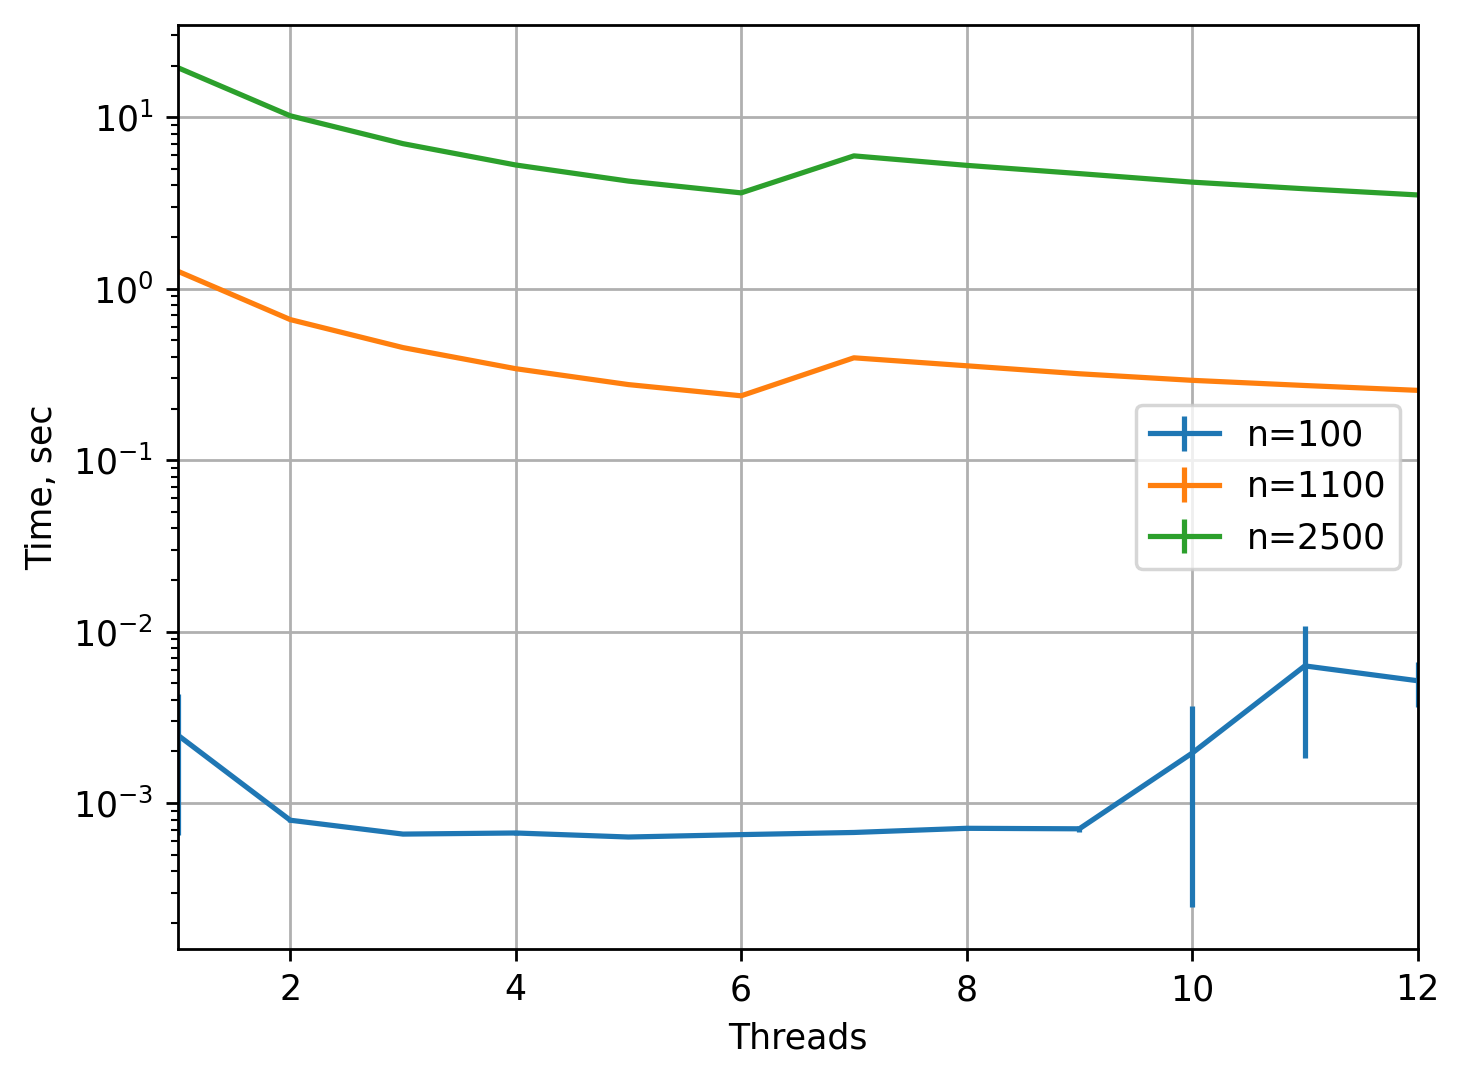
\includegraphics[scale=0.75]{t_vs_threads.png}
    \caption{Время выполнения оптимизированной программы в секундах при различном числе потоков. Показано среднее за 3 эксперимента время. Вертикальными линиями отмечены плюс и минус одно стандартное отклонение (корень из дисперсии)}
    \label{fig:t_vs_threads}
\end{figure}

\subsection{Ускорение алгоритма}

Чтобы определить ускорение, для каждого $n = 100,\; 1100,\; 2500$ вычисляется среднее время работы алгоритма в последовательном режиме $t^{(n)}_1$ с абсолютной погрешностью $\Delta t^(n)_1$, которая равна стандартному отклонению времени работы алгоритма в последовательном режиме. Далее считается само ускорение алгоритма с матрицей размера $n\times n$ для $T$ потоков по формуле
\begin{equation}
    k^{(n)}_T = \dfrac{t^{(n)}_1}{t^{(n)}_T},
\end{equation}
где $t^{(n)}_T$ --- среднее время работы алгоритма с матрицей размера $n\times n$ на $T$ потоках. Погрешность ускорения рассчитывается следующим образом:
\begin{equation}
   \Delta k^{(n)}_T = \dfrac{\Delta t^{(n)}_1 \cdot t^{(n)}_T + \Delta t^{(n)}_T \cdot t^{(n)}_1}{(t^{(n)}_T)^2}.
\end{equation}

На Рис. \ref{fig:speedup_vs_threads} показана зависимость ускорения от числа потоков при различной вычислительной сложности, закрашенные области соответствуют плюс и минус одному стандартному отклонению.
\begin{figure}[htbp]
    \centering
    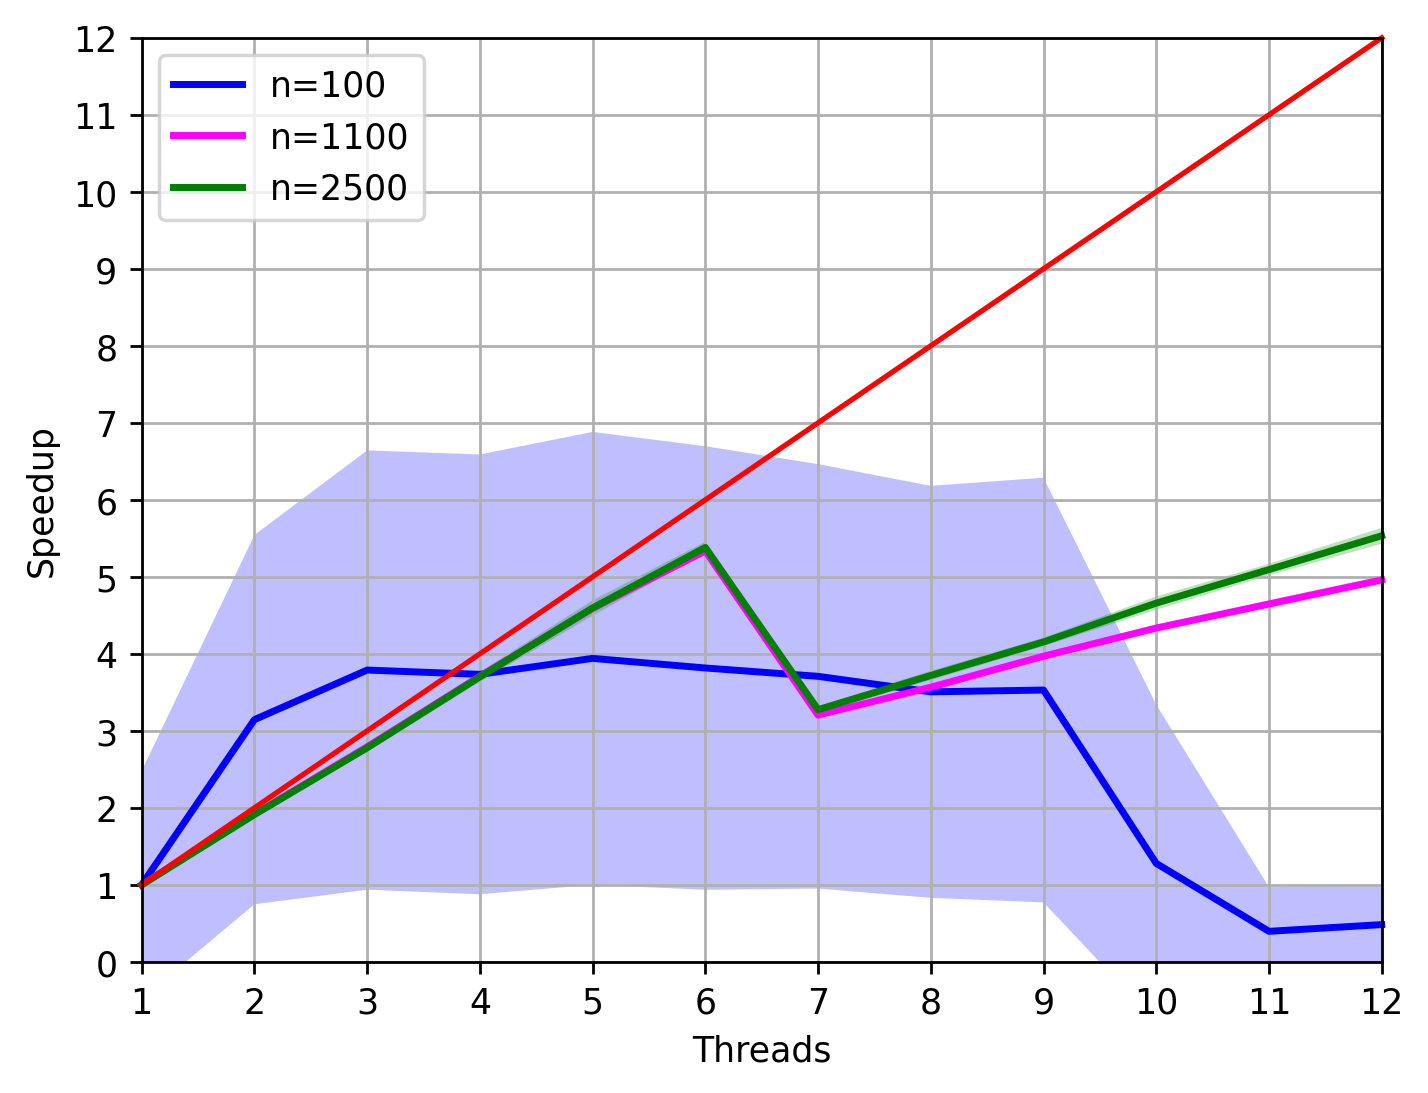
\includegraphics[scale=0.75]{speedup_vs_threads.png}
    \caption{Ускорение оптимизированной программы при различном числе потоков, закрашенные области соответствуют плюс и минус одному стандартному отклонению (для некоторых линий закрашенных областей может быть не видно, это свидетельствует лишь о малости ошибки). Красная линия обозначает идеальный случай, когда ускорение равно числу потоков.}
    \label{fig:speedup_vs_threads}
\end{figure}

\section{Интерпретация результатов, выводы}

При большой вычислительной сложности задачи, как видно на Рис. \ref{fig:speedup_vs_threads} для n=1100 и 2500, закон Амдала выполняется при числе потоков от 1 до 6, при этом удается достичь ускорения, близкого к числу потоков. Затем, при переходе от числа потоков, равного 6, к числу потоков, равному 7, происходит резкое падение ускорения. При дальнейшем увеличении числа потоков снова виден рост ускорения. Вероятно, падение ускорения при увеличении числа потоков от 6 до 7 связано с особенностями устройства вычислительной машины.

При малой вычислительной сложности задачи, как видно на Рис. \ref{fig:speedup_vs_threads} для n=100, трудно сделать выводы относительно выполнимости закона Амдала из-за большой погрешности определения ускорения. Однако, можно заметить, что при большом числе потоков видно уменьшение ускорения. Это можно связать с тем, что при малой сложности задачи на обмен информации между потоками тратится число операций, сравнимое с числом арифметических операций в задаче.

Таким образом, наиболее эффективно поддаются распараллеливанию задачи более трудоемкие ($n$ больше либо порядка 1000).

\newpage
\section*{Приложение}
\begin{lstlisting}[language=fortran, style=fortran, label={listing:3}, caption={Исходный код, оптимизированного с помощью OpenMP решателя системы \eqref{eq:1}, основанного на разложении Холецкого, на Фортране.}]
program linear_algebra_cholesky
   use omp_lib
   implicit none
   integer, parameter :: m = 10
   integer :: n
   real(4), allocatable :: a(:,:), l(:,:), l_t(:,:), id(:,:)
   real(4), allocatable :: b(:,:), x(:,:), y(:)
   integer :: i, j, ip
   real(8) :: time, s
   ! Reading n
   read(*, *) n
   ! Id matrix
   allocate(id(n,n))
   ForAll(i = 1:n, j = 1:n) id(i,j) = (i/j)*(j/i)
   ! Initialization of the matrix A
   allocate(a(n,n))
   call random_number(a)   
   a = (a + transpose(a)) / 2 + n * id
   ! Matrix b initialization
   allocate(b(n,m))
   b(:,:) = 1.0
   ! Initialization of a time counter
   time = omp_get_wtime()
   ! Cholesky decomposition
   allocate(l(n,n))
   l = a
   do  i = 1, n
      s = l(i,i)
      do  ip = 1, i - 1
         s = s - dprod(l(i,ip), l(i,ip))
      end do
      l(i,i) = sqrt(s)
      !$omp parallel do private(j,ip,s) shared(l,i) schedule(static)
      do  j = i + 1, n
         s = l(j,i)
         do  ip = 1, i-1
            s = s - dprod(l(i,ip), l(j,ip))
         end do
         l(j,i) = s / l(i,i)
      end do
      !$omp end parallel do
   end do
   ! back substitution
   allocate(l_t(n,n))
   l_t = transpose(l)
   allocate(y(n))
   allocate(x(n,m))
   !$omp parallel do private(i,j,y,s) shared(x,l,l_t) schedule(static)
   do i = 1, m
      y(1) = b(1,i) / l(1,1)
      do j = 2, n
         s = b(j,i)
         do ip = 1, j - 1
            s = s - dprod(l(j,ip), y(ip))
         end do
         y(j) = s / l(j,j)
      end do
      x(n,i) = y(n) / l_t(n,n)
      do j = n - 1, 1, -1
         s = y(j)
         do ip = j + 1, n
            s = s - dprod(l_t(j,ip), x(ip,i)) 
         end do
         x(j,i) = s / l_t(j,j)
      end do
   end do
   !$omp end parallel do
   ! Time
   time = omp_get_wtime() - time
   write(*,*) n, time
   deallocate(id)
   deallocate(a)
   deallocate(b)
   deallocate(l)
   deallocate(l_t)
   deallocate(y)
   deallocate(x)
end program linear_algebra_cholesky
\end{lstlisting}

% Please add the following required packages to your document preamble:
% \usepackage{multirow}
\begin{table}[htbp]
\begin{adjustbox}{angle=90}
\begin{tabular}{|c|ccc|ccc|ccc|}
\hline
\multirow{2}{*}{Threads \textbackslash n} & \multicolumn{3}{c|}{100} & \multicolumn{3}{c|}{1100} & \multicolumn{3}{c|}{2500} \\ \cline{2-10} 
 & \multicolumn{1}{c|}{Exp\#1} & \multicolumn{1}{c|}{Exp\#2} & Exp\#2 & \multicolumn{1}{c|}{Exp\#1} & \multicolumn{1}{c|}{Exp\#2} & Exp\#3 & \multicolumn{1}{c|}{Exp\#1} & \multicolumn{1}{c|}{Exp\#2} & Exp\#3 \\ \hline
1 & \multicolumn{1}{c|}{5.11e-03} & \multicolumn{1}{c|}{1.17e-03} & 1.21e-03 & \multicolumn{1}{c|}{1.27e+00} & \multicolumn{1}{c|}{1.26e+00} & 1.26e+00 & \multicolumn{1}{c|}{1.97e+01} & \multicolumn{1}{c|}{1.92e+01} & 1.95e+01 \\ \hline
2 & \multicolumn{1}{c|}{7.93e-04} & \multicolumn{1}{c|}{8.16e-04} & 7.73e-04 & \multicolumn{1}{c|}{6.59e-01} & \multicolumn{1}{c|}{6.63e-01} & 6.59e-01 & \multicolumn{1}{c|}{1.02e+01} & \multicolumn{1}{c|}{1.02e+01} & 1.01e+01 \\ \hline
3 & \multicolumn{1}{c|}{6.58e-04} & \multicolumn{1}{c|}{6.70e-04} & 6.49e-04 & \multicolumn{1}{c|}{4.49e-01} & \multicolumn{1}{c|}{4.58e-01} & 4.53e-01 & \multicolumn{1}{c|}{6.95e+00} & \multicolumn{1}{c|}{7.08e+00} & 6.99e+00 \\ \hline
4 & \multicolumn{1}{c|}{6.73e-04} & \multicolumn{1}{c|}{6.87e-04} & 6.47e-04 & \multicolumn{1}{c|}{3.39e-01} & \multicolumn{1}{c|}{3.43e-01} & 3.43e-01 & \multicolumn{1}{c|}{5.29e+00} & \multicolumn{1}{c|}{5.21e+00} & 5.29e+00 \\ \hline
5 & \multicolumn{1}{c|}{6.32e-04} & \multicolumn{1}{c|}{6.39e-04} & 6.31e-04 & \multicolumn{1}{c|}{2.78e-01} & \multicolumn{1}{c|}{2.75e-01} & 2.75e-01 & \multicolumn{1}{c|}{4.19e+00} & \multicolumn{1}{c|}{4.22e+00} & 4.31e+00 \\ \hline
6 & \multicolumn{1}{c|}{6.49e-04} & \multicolumn{1}{c|}{6.68e-04} & 6.46e-04 & \multicolumn{1}{c|}{2.38e-01} & \multicolumn{1}{c|}{2.36e-01} & 2.38e-01 & \multicolumn{1}{c|}{3.63e+00} & \multicolumn{1}{c|}{3.60e+00} & 3.62e+00 \\ \hline
7 & \multicolumn{1}{c|}{6.74e-04} & \multicolumn{1}{c|}{6.76e-04} & 6.71e-04 & \multicolumn{1}{c|}{3.97e-01} & \multicolumn{1}{c|}{3.91e-01} & 3.97e-01 & \multicolumn{1}{c|}{5.97e+00} & \multicolumn{1}{c|}{5.93e+00} & 5.94e+00 \\ \hline
8 & \multicolumn{1}{c|}{7.33e-04} & \multicolumn{1}{c|}{7.12e-04} & 6.93e-04 & \multicolumn{1}{c|}{3.53e-01} & \multicolumn{1}{c|}{3.58e-01} & 3.54e-01 & \multicolumn{1}{c|}{5.28e+00} & \multicolumn{1}{c|}{5.22e+00} & 5.21e+00 \\ \hline
9 & \multicolumn{1}{c|}{7.07e-04} & \multicolumn{1}{c|}{7.44e-04} & 6.72e-04 & \multicolumn{1}{c|}{3.19e-01} & \multicolumn{1}{c|}{3.18e-01} & 3.20e-01 & \multicolumn{1}{c|}{4.71e+00} & \multicolumn{1}{c|}{4.68e+00} & 4.68e+00 \\ \hline
10 & \multicolumn{1}{c|}{4.37e-03} & \multicolumn{1}{c|}{7.55e-04} & 7.40e-04 & \multicolumn{1}{c|}{2.92e-01} & \multicolumn{1}{c|}{2.91e-01} & 2.93e-01 & \multicolumn{1}{c|}{4.23e+00} & \multicolumn{1}{c|}{4.14e+00} & 4.17e+00 \\ \hline
11 & \multicolumn{1}{c|}{6.11e-03} & \multicolumn{1}{c|}{9.19e-04} & 1.19e-02 & \multicolumn{1}{c|}{2.75e-01} & \multicolumn{1}{c|}{2.70e-01} & 2.72e-01 & \multicolumn{1}{c|}{3.80e+00} & \multicolumn{1}{c|}{3.85e+00} & 3.82e+00 \\ \hline
12 & \multicolumn{1}{c|}{5.31e-03} & \multicolumn{1}{c|}{3.24e-03} & 6.96e-03 & \multicolumn{1}{c|}{2.53e-01} & \multicolumn{1}{c|}{2.56e-01} & 2.57e-01 & \multicolumn{1}{c|}{3.50e+00} & \multicolumn{1}{c|}{3.56e+00} & 3.50e+00 \\ \hline
\end{tabular}
\end{adjustbox}
\caption{Время работы программы в секундах при различном числе потоков (Threads) и числе столбцов матрицы $\vb{A}$ $n$. Приведены результаты трёх численных экспериментов для каждого $n$.}
\label{tab:2}
\end{table}


\end{document}
